\section{System Architecture}\label{sec:architecture}

The cell sorts three part types arriving on a moving conveyor into six bins: one bin per good
type (Type~A, B, C) plus Rework, Scrap and Quarantine. A 6-axis articulated arm with a suction
gripper picks each part from the moving belt. There is no hardware: the plant is a MuJoCo
digital twin (Section~\ref{sec:twin}), and the controller is a CODESYS soft-PLC running an
IEC~61131-3 application~\cite{IEC61131-3}.

\subsection{Layers and Real-Time Boundaries}

The system is split into layers with different time scales (Fig.~\ref{fig:architecture}). One
rule connects them: a slower layer never blocks a faster one. The PLC never waits for vision or
for the decision layer. If a vision result is missing, the part is not picked; if a decision is
late, the PLC applies its own rule.

\begin{figure}[t]
\centering
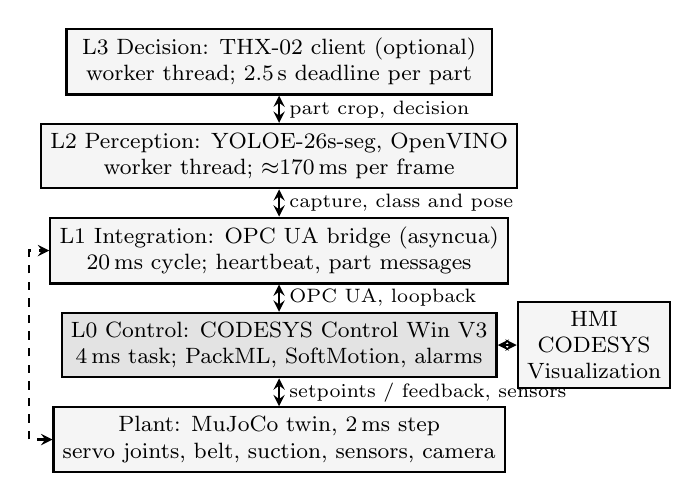
\begin{tikzpicture}[
    font=\footnotesize,
    layer/.style={draw, thick, rectangle, minimum width=5.4cm, minimum height=0.8cm,
                  align=center, fill=gray!8},
    plc/.style={layer, fill=gray!22},
    side/.style={draw, thick, rectangle, minimum width=1.5cm, minimum height=0.85cm,
                 align=center, fill=gray!8},
    arr/.style={<->, >=stealth, thick}]
  \node[layer] (l3) at (0,4.8) {L3 Decision: THX-02 client (optional)\\worker thread; 2.5\,s deadline per part};
  \node[layer] (l2) at (0,3.6) {L2 Perception: YOLOE-26s-seg, OpenVINO\\worker thread; $\approx$170\,ms per frame};
  \node[layer] (l1) at (0,2.4) {L1 Integration: OPC UA bridge (asyncua)\\20\,ms cycle; heartbeat, part messages};
  \node[plc]   (l0) at (0,1.2) {L0 Control: CODESYS Control Win V3\\4\,ms task; PackML, SoftMotion, alarms};
  \node[layer] (pl) at (0,0.0) {Plant: MuJoCo twin, 2\,ms step\\servo joints, belt, suction, sensors, camera};
  \node[side]  (hmi) at (4.0,1.2) {HMI\\CODESYS\\Visualization};
  \draw[arr] (l3) -- node[right, font=\scriptsize] {part crop, decision} (l2);
  \draw[arr] (l2) -- node[right, font=\scriptsize] {capture, class and pose} (l1);
  \draw[arr] (l1) -- node[right, font=\scriptsize] {OPC UA, loopback} (l0);
  \draw[arr] (l0) -- node[right, font=\scriptsize] {setpoints / feedback, sensors} (pl);
  \draw[arr] (l0) -- (hmi);
  \draw[<->, >=stealth, thick, dashed] (pl.west) -- ++(-0.3,0) |- (l1.west);
\end{tikzpicture}
\caption{Control layers of the cell. The PLC (L0) is master of motion; the twin is master of
physical objects. Solid arrows show the logical data flow. The bridge and the twin run in one
Python process, so the PLC's exchange with the twin passes through the 20\,ms bridge cycle
(dashed).}
\label{fig:architecture}
\end{figure}

\subsection{Who Is Master of What}

Joint setpoints, the tool centre point (TCP) pose and the conveyor position are owned by the PLC:
the robot axes and the conveyor are SoftMotion virtual drives that generate setpoints. The twin
does not copy them. Each joint is a simulated servo drive that tracks the setpoint and reports
its measured position and torque back. The 20\,ms OPC UA link cannot close a servo loop, so the
servo loop lives in the twin, as it would in a real drive, and the PLC does trajectory generation
and supervision. Physical objects (parts on the belt, in the gripper, in the bins) are owned by
the twin; the PLC learns their state only through simulated sensors (photo-eyes, vacuum switch,
bin-full signals, door, E-stop). Class and pose come from vision and, optionally, quality from the
decision layer; once written into the PLC's part record, the PLC owns them.

\subsection{Life of a Part}

The twin spawns a part upstream. When the part interrupts photo-eye PE1, the PLC latches the belt
position, assigns a part id and publishes a capture request. The vision worker renders the camera
image and returns the part's class, confidence and pose $(x, y, \theta)$ in the belt frame at the
capture. If a decision service is configured, it adds a quality disposition and an
identification-reliability answer. The PLC selects the bin, waits until the part is inside the
pick window, tracks it with the robot, picks it with suction and places it in the bin.

\subsection{PLC--Python Interface}

The PLC and the Python services exchange data over OPC UA~\cite{IEC62541}. The CODESYS OPC UA
server publishes only two global variable lists: \texttt{GVL\_Bridge} (setpoints, feedback,
sensors, part messages, diagnostics) and \texttt{GVL\_Hmi} (operator commands). Tag names have a
single source of truth, \texttt{config/opcua\_tags.yaml}. Every message structure carries a
sequence number that the bridge writes last and that the PLC uses to accept each message exactly
once (\texttt{FB\_MessageIntake}). The bridge toggles a heartbeat every cycle; if the PLC sees no
change for 500\,ms it raises a critical alarm and the cell aborts. The endpoint is anonymous and
unencrypted but bound to the loopback interface, with the runtime's inbound firewall rules
disabled. This is acceptable only for a single-host laboratory cell; a plant would use signed and
encrypted sessions.
